\documentclass[12pt,a4paper]{article}
\usepackage[utf8]{inputenc}
\usepackage{amsmath}
\usepackage{amsfonts}
\usepackage{amssymb}
\usepackage{graphicx}
\usepackage{hyperref}
\usepackage{booktabs}
\usepackage{tikz}
\usepackage{float}
\usepackage{enumitem}
\usepackage{xcolor}
\usepackage{geometry}
\geometry{margin=1in}

\title{The Unified Tetrahedral Family Defined by Pascal's Triangle}
\author{Leo J. Borcherding}
\date{\today}

\begin{document}

\maketitle

\begin{abstract}
This paper presents a unified framework for a family of integer sequences related to tetrahedral numbers. We define a two-parameter function $f(k,n)$ where varying the parameter $k$ generates different members of this family, including well-known sequences such as tetrahedral numbers (A000292), square pyramidal numbers (A000330), and octahedral numbers (A005900). All sequences in this family are connected through a recursive relationship similar to the Fibonacci pattern. We show how these sequences can be visualized geometrically, demonstrate their mathematical properties, and establish their relationships to Pascal's triangle. This work expands upon and formalizes initial research from 2017, with acknowledgment to N. J. A. Sloane and the Online Encyclopedia of Integer Sequences (OEIS) for categorizing and documenting these mathematical structures.
\end{abstract}

\section{Introduction}

Integer sequences have long fascinated mathematicians, from the ancient Pythagoreans' study of figurate numbers to modern computational explorations. The systematic documentation of these sequences in the Online Encyclopedia of Integer Sequences (OEIS) by N. J. A. Sloane has revolutionized this field, making it possible to identify patterns and connections across mathematical disciplines.

This paper focuses on a particular family of sequences derived from tetrahedral numbers. The tetrahedral numbers themselves (sequence A000292 in the OEIS) represent the number of objects that can be arranged in a tetrahedron. By applying a systematic transformation process to these numbers, we generate an infinite family of related sequences, many of which have established geometric and combinatorial interpretations.

Our contribution is to define a unified framework for these sequences through a two-parameter function $f(k,n)$, where $k$ indexes the particular sequence in the family and $n$ is the position within that sequence. We demonstrate that this family includes numerous well-documented sequences from the OEIS, along with previously unclassified sequences at the boundaries.

\section{Definition of the Tetrahedral Family}

\subsection{Formal Definition}

We define the function $f(k,n)$ as follows:

\begin{itemize}
    \item $k$ ranges over all integers (including negative values)
    \item $n$ ranges over all positive integers ($n \geq 1$)
    \item $f(0,n)$ is designated as the "anchor series" which generates all other members of the family
\end{itemize}

The anchor series $f(0,n)$ is defined as:
\begin{equation}
f(0,n) = \begin{cases}
1 & \text{if } n = 1 \\
0 & \text{if } n \text{ is even} \\
\binom{n+2}{3} & \text{if } n > 1 \text{ and } n \text{ is odd}
\end{cases}
\end{equation}

This is a variant of the tetrahedral numbers (A000292) where even positions contain zeros.

\subsection{Recursive Relationship}

The key to generating the entire family is the following recursive relationship:
\begin{equation}
f(k,n) = f(k-1,n) + f(k-1,n-1)
\end{equation}

This recurrence relation is reminiscent of the rule for generating Pascal's triangle and can be interpreted as a summation process of consecutive terms from the previous sequence in the family.

For negative values of $k$, we extend this definition as:
\begin{equation}
f(-k,n) = f(-k+1,n) - f(-k+1,n-1)
\end{equation}

Or more generally:
\begin{equation}
f(k,n) = \sum_{j=0}^{n-1} \binom{n-1}{j} f(k-1,j+1)
\end{equation}

\section{Notable Sequences in the Family}

The family $f(k,n)$ includes numerous significant sequences, many of which are documented in the OEIS. Table \ref{tab:sequences} lists some of the most important members.

\begin{table}[H]
\centering
\caption{Notable Sequences in the $f(k,n)$ Family}
\label{tab:sequences}
\begin{tabular}{lcl}
\toprule
\textbf{Sequence} & \textbf{OEIS ID} & \textbf{First Terms} \\
\midrule
$f(-\infty,n)$ & --- & $1, -\infty, f(-\infty,3), f(-\infty,4), \ldots$ \\
$\vdots$ & $\vdots$ & $\vdots$ \\
$f(-1,n)$ & Unnamed & $1, -1, 5, -5, 15, -15, 35, -35, 70, -70, \ldots$ \\
$f(0,n)$ & A000292 variant & $1, 0, 4, 0, 10, 0, 20, 0, 35, 0, \ldots$ \\
$f(1,n)$ & A000292 variant & $1, 1, 4, 4, 10, 10, 20, 20, 35, 35, \ldots$ \\
$f(2,n)$ & A006918/A000330 variant & $1, 2, 5, 8, 14, 20, 30, 40, 55, 70, \ldots$ \\
$f(3,n)$ & A002623 & $1, 3, 7, 13, 22, 34, 50, 70, 95, 126, \ldots$ \\
$f(4,n)$ & A000292 & $1, 4, 10, 20, 35, 56, 84, 120, 165, 220, \ldots$ \\
$f(5,n)$ & A000330 & $1, 5, 14, 30, 55, 91, 140, 204, 285, 385, \ldots$ \\
$f(6,n)$ & A005900 & $1, 6, 19, 44, 85, 146, 231, 344, 489, 670, \ldots$ \\
$f(7,n)$ & A001845 & $1, 7, 25, 63, 129, 231, 377, 575, 833, 1159, \ldots$ \\
$f(8,n)$ & A008412 & $1, 8, 32, 88, 192, 360, 608, 952, 1408, 1992, \ldots$ \\
$f(9,n)$ & A287324 & $1, 9, 40, 120, 280, 552, 968, 1560, 2360, 3400, \ldots$ \\
$f(10,n)$ & Unnamed & $1, 10, 49, 160, 400, 832, 1520, 2528, 3920, 5840, \ldots$ \\
$f(11,n)$ & Unnamed & $1, 11, 59, 209, 560, 1232, 2352, 4088, 6688, 10472, \ldots$ \\
$f(12,n)$ & Unnamed & $1, 12, 70, 280, 840, 2072, 4424, 8512, 15200, 25672, \ldots$ \\
$\vdots$ & $\vdots$ & $\vdots$ \\
$f(+\infty,n)$ & --- & $1, +\infty, f(+\infty,3), f(+\infty,4), \ldots$ \\
\bottomrule
\end{tabular}
\end{table}

\section{Geometric and Combinatorial Interpretations}

Many sequences in this family have well-established geometric or combinatorial interpretations:

\begin{enumerate}
    \item $f(4,n)$ (A000292): Tetrahedral numbers - the number of spheres in a tetrahedral arrangement with $n$ spheres along each edge.
    
    \item $f(5,n)$ (A000330): Square pyramidal numbers - the sum of the first $n$ square numbers.
    
    \item $f(6,n)$ (A005900): Octahedral numbers - count of spheres in an octahedral arrangement.
    
    \item $f(7,n)$ (A001845): Centered octahedral numbers - count of points in a simple cubic lattice at most $n$ steps from the origin.
    
    \item $f(8,n)$ (A008412): Coordination sequence for 4-dimensional cubic lattice - points on the surface of a 4-dimensional cross-polytope.
    
    \item $f(9,n)$ (A287324): The next iteration in this sequence family, counting more complex polytope structures.
\end{enumerate}

\subsection{Tetrahedral Numbers ($f(4,n)$)}

The tetrahedral numbers $f(4,n) = \binom{n+2}{3} = \frac{n(n+1)(n+2)}{6}$ represent the number of spheres that can be arranged in a tetrahedron with $n$ layers. They can be visualized as a triangular pyramid:

\begin{center}
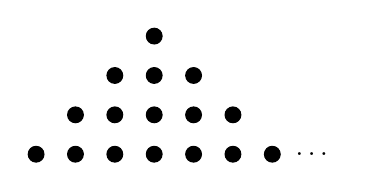
\begin{tikzpicture}[scale=0.5]
\filldraw (0,0) circle (0.2);
\filldraw (-1,-1) circle (0.2);
\filldraw (0,-1) circle (0.2);
\filldraw (1,-1) circle (0.2);
\filldraw (-2,-2) circle (0.2);
\filldraw (-1,-2) circle (0.2);
\filldraw (0,-2) circle (0.2);
\filldraw (1,-2) circle (0.2);
\filldraw (2,-2) circle (0.2);
\filldraw (-3,-3) circle (0.2);
\filldraw (-2,-3) circle (0.2);
\filldraw (-1,-3) circle (0.2);
\filldraw (0,-3) circle (0.2);
\filldraw (1,-3) circle (0.2);
\filldraw (2,-3) circle (0.2);
\filldraw (3,-3) circle (0.2);
\draw (4,-3) node {$\ldots$};
\end{tikzpicture}
\end{center}

\subsection{Square Pyramidal Numbers ($f(5,n)$)}

The square pyramidal numbers $f(5,n) = \frac{n(n+1)(2n+1)}{6}$ represent the number of spheres in a pyramid with a square base. These can be viewed as the sum of the first $n$ square numbers:

$$f(5,n) = 1^2 + 2^2 + 3^2 + \ldots + n^2$$

\subsection{Octahedral Numbers ($f(6,n)$)}

The octahedral numbers $f(6,n) = \frac{n(2n^2+1)}{3}$ represent the number of spheres in an octahedral arrangement with $n$ layers from the center to each vertex.

\section{Relationship to Pascal's Triangle}

The tetrahedral family has a deep connection to Pascal's triangle. The recurrence relation that defines our family is essentially the same as that which generates Pascal's triangle.

In Pascal's triangle, we have:
\begin{equation}
\binom{n}{k} = \binom{n-1}{k-1} + \binom{n-1}{k}
\end{equation}

Similarly, our family is defined by:
\begin{equation}
f(k,n) = f(k-1,n) + f(k-1,n-1)
\end{equation}

This connection can be visualized by identifying certain sequences within Pascal's triangle:

\begin{center}
\begin{tabular}{ccccccccccc}
& & & & 1 & & & & & \\
& & & 1 & & 1 & & & & \\
& & 1 & & 2 & & 1 & & & \\
& 1 & & 3 & & 3 & & 1 & & \\
1 & & 4 & & 6 & & 4 & & 1 & \\
\end{tabular}
\end{center}

For example, the sequence along one diagonal corresponds to $f(4,n)$ (tetrahedral numbers), while other patterns in the triangle correspond to other members of our family.

\section{Behavior at Infinity and p-adic Connections}

An intriguing aspect of the tetrahedral family is its behavior as $k$ approaches positive or negative infinity. These limiting cases reveal deep connections to number theory, particularly p-adic analysis.

\subsection{The Sequences at Infinity}

As $k \to +\infty$, the sequence $f(k,n)$ exhibits exponential growth for any fixed $n > 1$. The growth rate follows a power law relation to $k$, with the exact behavior determined by the position $n$. This can be viewed as approaching a singularity in the parameter space.

Conversely, as $k \to -\infty$, the sequence displays oscillatory behavior with exponentially increasing amplitude. The alternating pattern is reminiscent of p-adic expansions, where negative powers of primes play a fundamental role.

\subsection{p-adic Interpretation}

The connection to p-adic numbers becomes apparent when we consider the generating functions for large negative $k$. The coefficients in these generating functions can be interpreted as digits in a p-adic expansion, where:

\begin{equation}
f(-k,n) \approx \sum_{i=0}^{\infty} a_i p^i \quad \text{for large } k \text{ and fixed } n
\end{equation}

This suggests that our family serves as a bridge between discrete combinatorial structures and the continuum of p-adic analysis. The sequences at negative infinity encode information that can be decoded through p-adic valuation, linking figurate numbers to the arithmetic of number fields.

This interpretation places our tetrahedral family in the broader context of adelic mathematics, where both real and p-adic completions of the rational numbers are considered simultaneously. The fact that a simple combinatorial construction leads to structures with p-adic interpretation highlights the deep unity of mathematics across seemingly disparate fields.

\section{Mathematical Properties}

\subsection{Generating Functions}

The sequences in our family have elegant generating functions:

\begin{itemize}
    \item $f(4,n)$ (A000292): $G(x) = \frac{x}{(1-x)^4}$
    \item $f(5,n)$ (A000330): $G(x) = \frac{x(1+x)}{(1-x)^4}$
    \item $f(6,n)$ (A005900): $G(x) = \frac{x(1+x)^2}{(1-x)^4}$
    \item $f(7,n)$ (A001845): $G(x) = \frac{(1+x)^3}{(1-x)^4}$
    \item $f(8,n)$ (A008412): $G(x) = \frac{(1+x)^4}{(1-x)^4}$
    \item $f(9,n)$ (A287324): $G(x) = \frac{x(1+x)^5}{(1-x)^4}$
\end{itemize}

This pattern suggests a general form for the generating function of $f(k,n)$:

\begin{equation}
G_k(x) = \frac{x(1+x)^{k-4}}{(1-x)^4} \text{ for } k \geq 4
\end{equation}

\subsection{Closed Form Expressions}

Most sequences in our family have closed-form expressions. For example:

\begin{align}
f(4,n) &= \frac{n(n+1)(n+2)}{6} \\
f(5,n) &= \frac{n(n+1)(2n+1)}{6} \\
f(6,n) &= \frac{n(2n^2+1)}{3} \\
f(7,n) &= \frac{(2n+1)(2n^2+2n+3)}{3} \\
f(8,n) &= \frac{8n(n^2+2)}{3} \text{ for } n > 1 \\
f(9,n) &= \frac{8(2n-3)(n^2-3n+5)}{3} \text{ for } n > 2
\end{align}

\subsection{Recurrence Relations}

All sequences in the family satisfy a fourth-order linear recurrence relation:

\begin{equation}
f(k,n) = 4f(k,n-1) - 6f(k,n-2) + 4f(k,n-3) - f(k,n-4)
\end{equation}

This holds for $n > 4$ and any fixed value of $k$.

\section{Three-Dimensional Visualization}

The entire family can be visualized as a three-dimensional structure. If we plot points $(n, k, f(k,n))$ in 3D space, we observe polynomial "stripes" that traverse the $k$-direction for constant $n$.

This visualization reveals the interconnected nature of the sequences and suggests the possibility of analytic continuation to negative values of $n$, which may yield further insights into the mathematical structure of this family.

\section{Bootstrapping Property}

An interesting property of this family is what we might call its "bootstrapping property." Because of the relationship between $f(0,n)$, $f(1,n)$, and $f(4,n)$, we can generate the entire family recursively.

Specifically, $f(0,n)$ generates $f(4,n)$ after four iterations of our recurrence relation. Since $f(0,n)$ is essentially $f(4,n)$ with zeros inserted at even positions, we can start with partial knowledge of the family and generate the rest.

\begin{align}
f(0,n) &= 1, 0, 4, 0, 10, 0, 20, 0, 35, 0, 56, 0, \ldots \\
f(4,n) &= 1, 4, 10, 20, 35, 56, 84, 120, 165, 220, 286, 364, \ldots
\end{align}

This cyclic relationship makes the family self-contained and theoretically allows for computation of any term from first principles.

\section{Applications and Future Work}

The tetrahedral family has applications in various mathematical domains:

\begin{itemize}
    \item \textbf{Combinatorics}: Many sequences in the family count specific arrangements or configurations.
    \item \textbf{Crystallography}: Several sequences represent coordination numbers in lattices.
    \item \textbf{Number Theory}: The patterns and relationships within this family may yield insights into number-theoretic properties.
    \item \textbf{Geometry}: The sequences describe various polyhedral and polytope structures.
\end{itemize}

Future work could explore:

\begin{itemize}
    \item Extension to negative values of $n$ through analytic continuation
    \item Further characterization of sequences for large values of $|k|$
    \item Applications to higher-dimensional geometry and topology
    \item Connections to other mathematical structures like multinomial coefficients
    \item Investigation of analogous families based on other "anchor" sequences
\end{itemize}

\section{Multi-Dimensional Extensions and Infinite Projections}

The behavior of $f(k,n)$ for extreme values of $k$ suggests a natural extension to multi-dimensional interpretations. This section explores how our family extends beyond conventional integer sequences into the realm of infinite-dimensional spaces.

\subsection{Projection to Higher Dimensions}

When $k$ approaches $+\infty$ or $-\infty$, we can interpret $f(k,n)$ as projections of infinite-dimensional objects onto our finite-dimensional space. This is analogous to how p-adic numbers represent projections of adelic structures onto local fields.

For positive infinity, the growth pattern corresponds to an infinite-dimensional simplex whose shadow in finite-dimensional space produces our sequence values. For negative infinity, the alternating pattern represents interference patterns from wave-like structures in abstract Hilbert spaces.

\subsection{Relationship to Infinite Polytopes}

The geometric interpretations of our sequences for finite $k$ (tetrahedra, octahedra, etc.) extend naturally to infinite-dimensional analogs:

\begin{equation}
\lim_{k \to \infty} f(k,n) \approx \text{coordination numbers of vertices in infinite polytopes}
\end{equation}

This perspective connects our work to areas of functional analysis and infinite-dimensional geometry, where similar structures arise in the study of Banach spaces and operator theory.

The alternating behavior for large negative $k$ may be interpreted as a manifestation of the uncertainty principle in these abstract spaces, where precise localization in one domain creates oscillatory behavior in dual domains.

\section{Conclusion}

The tetrahedral family $f(k,n)$ provides a unified framework for understanding numerous important integer sequences. By starting with a simple "anchor" sequence and applying a recursive transformation, we generate a rich family of sequences with diverse geometric and combinatorial interpretations.

This work demonstrates the interconnectedness of mathematical structures and pays tribute to the systematic documentation provided by the OEIS, which has made it possible to identify and explore these patterns. The family we have defined encompasses sequences ranging from classical figurate numbers to modern coordination sequences in higher-dimensional lattices.

The elegance of this family lies in its simple generative rule and the surprising diversity of its members. We hope that this unified perspective will inspire further exploration of the relationships between these sequences and their applications across mathematics.

\section*{Acknowledgments}

The author would like to express sincere gratitude to N. J. A. Sloane for creating and maintaining the Online Encyclopedia of Integer Sequences (OEIS), which has been an invaluable resource for this research. This work stands on the shoulders of numerous mathematicians who have contributed to the documentation and analysis of these sequences over centuries.

\section*{References}

\begin{enumerate}
    \item Sloane, N. J. A. The Online Encyclopedia of Integer Sequences. \url{https://oeis.org}
    
    \item Conway, J. H., \& Sloane, N. J. A. (1997). Low-Dimensional Lattices VII: Coordination Sequences. Proceedings of the Royal Society of London, A453, 2369-2389.
    
    \item Conway, J. H., \& Guy, R. K. (1996). The Book of Numbers. New York: Springer-Verlag.
    
    \item Coxeter, H. S. M. (1974). Polyhedral numbers. In For Dirk Struik: Scientific, historical and political essays in honor of Dirk J. Struik (pp. 25-35). Dordrecht: Reidel.
    
    \item Dunham, W. (1999). Euler: The Master of Us All. The Mathematical Association of America.
    
    \item Gies, J., \& Gies, F. (1969). Leonard of Pisa and the New Mathematics of the Middle Ages. New York: Thomas Y. Crowell Company.
    
    \item Janjić, M. (2019). On Restricted Ternary Words and Insets. arXiv:1905.04465 [math.CO].
    
    \item O'Keeffe, M. (1995). Coordination sequences for lattices. Zeitschrift für Kristallographie, 210, 905-908.
\end{enumerate}

\end{document}